%%%%%%%%%%%%%%%%%%%%%%%%%%%%%%%%%%%%%%%%%
% Simple Sectioned Essay Template
% LaTeX Template
%
% This template has been downloaded from:
% http://www.latextemplates.com
%
% Note:
% The \lipsum[#] commands throughout this template generate dummy text
% to fill the template out. These commands should all be removed when 
% writing essay content.
%
%%%%%%%%%%%%%%%%%%%%%%%%%%%%%%%%%%%%%%%%%

%----------------------------------------------------------------------------------------
%	PACKAGES AND OTHER DOCUMENT CONFIGURATIONS
%----------------------------------------------------------------------------------------

\documentclass[12pt]{article} % Default font size is 12pt, it can be changed here

\usepackage{geometry} % Required to change the page size to A4
\geometry{a4paper} % Set the page size to be A4 as opposed to the default US Letter

\usepackage{graphicx} % Required for including pictures

\usepackage[utf8]{inputenc}

\usepackage{float} % Allows putting an [H] in \begin{figure} to specify the exact location of the figure
%\usepackage{wrapfig} % Allows in-line images such as the example fish picture

\usepackage{lipsum} % Used for inserting dummy 'Lorem ipsum' text into the template

\usepackage{hyperref}
\usepackage{pdfpages}
\usepackage[toc,page]{appendix}
\usepackage{enumitem}
\usepackage{makecell}
\usepackage{color}

\linespread{1.2} % Line spacing

%\setlength\parindent{0pt} % Uncomment to remove all indentation from paragraphs

%\graphicspath{{Pictures/}} % Specifies the directory where pictures are stored

\begin{document}

%----------------------------------------------------------------------------------------
%	TITLE PAGE
%----------------------------------------------------------------------------------------

\begin{titlepage}

\newcommand{\HRule}{\rule{\linewidth}{0.5mm}} % Defines a new command for the horizontal lines, change thickness here

\center % Center everything on the page

\textsc{\LARGE KTH Royal Institute of Technology}\\[1.5cm] % Name of your university/college
\textsc{\Large Machine Department}\\[0.5cm] % Major heading such as course name


\HRule \\[0.4cm]
{ \huge \bfseries Project Plan of IDIOM Group}\\[0.4cm] % Title of your document
\HRule \\[1.5cm]

\begin{minipage}{0.4\textwidth}
\begin{flushleft} \large
\emph{Authors:}\\
Anqing \textsc{Duan}\\
Alexander \textsc{Gratner}\\
Yuchao \textsc{Li}
 % Your name
\end{flushleft}
\end{minipage}
~
\begin{minipage}{0.4\textwidth}
\begin{flushright} \large
\emph{Supervisor:} \\
Dr. Jad \textsc{El-Khoury}\\
Assoc. Prof. Lei \textsc{Feng} % Supervisor's Name
\end{flushright}
\end{minipage}\\[1cm]

\begin{figure}[!h]
  \centering
%    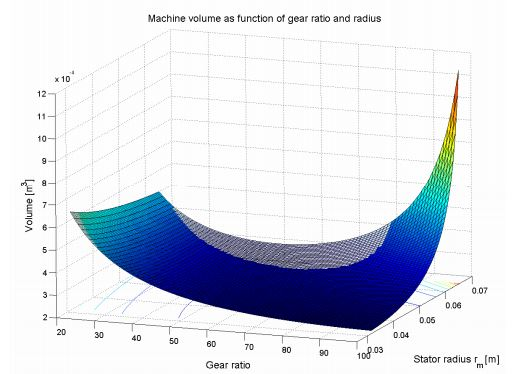
\includegraphics[width=0.7\textwidth]{Pictures/cover.jpg}

      \label{fig:Triangulation}
\end{figure}

\begin{minipage}{0.4\textwidth}
\end{minipage}\\[1cm]
{\large \today}\\[3cm] % Date, change the \today to a set date if you want to be precise

%\includegraphics{Logo}\\[1cm] % Include a department/university logo - this will require the graphicx package

\vfill % Fill the rest of the page with whitespace

\end{titlepage}



\newpage % Begins the essay on a new page instead of on the same page as the table of contents 

%----------------------------------------------------------------------------------------
%	INTRODUCTION
%----------------------------------------------------------------------------------------

\section{Preliminary Title} % Major section

This section presents the key words of the research and preliminary title.

\subsection{Key Words} 
There has been an agreement reached within the group that the title should indicate both the research context and mathematical tool. Therefore \textit{mechatronic system} and \textit{convex optimization} should be included in the title. Since the purpose of research is mainly focus on the modification of optimization algorithms, \textit{methodology} has not been included in the title.
 
\subsection{Title}
The preliminary title at this stage is \textit{Convex Optimization for Mechatronic System Design}.

%------------------------------------------------

%----------------------------------------------------------------------------------------
%	BACKGROUND
%----------------------------------------------------------------------------------------

\section{Background and Problem Description} % Major section

This section presents the background and purpose to the research. The research question is formulated in the end.

\subsection{Backgroud}
The target of the research is to explore the possibility of increasing the efficiency of one specific mechatronic design method by introducing new algorithm into the IDIOM software. The background is divided into two sections, one focusing on the design method of mechatornic systems and one focusing on genetic as well as convex algorithms.

\subsubsection{Integrated Design and Optimization of Mechatronic Products}
The development process of mechatronic products is challenging because it involves multiple engineering domains. In order to deal with them in an integrated manner as early as possible, several generic methodologies have been created, such as \textit{V-model} and \textit{Ulrich and Eppinger's model}. V-model, presented in \cite{VDI}, features frequent verification and validation against the requirements during the integration phases. Ulrich and Eppinger's model can be adopted in accordance with an unique context \cite{Ulrich}.

Although these methods have different formats, they do share something in common. According to \cite{VDI} and \cite{Ulrich}, the detailed design is carried out based on rather abstract design in early phase, which means if some problems occur, chances are that the design in early stages needs to be modified as well. Moreover the lack of knowledge in early phase makes this kind of trace back inevitable \cite{Holistic}. To aid this issue, the \textit{Integrated Design and Optimization of Mechatronic Products} (\textit{IDIOM}) method has been created to explore the potential of concept design with limited information.

The IDIOM method treats the mechatronic system in a holistic pattern,  integrating different domains in early design phase and optimizing parameters of designed structure with respect to one or multiple targets. Fredrik Roos contributed to the models of the method \cite{Roos} and Malmquist et al. extended the capability of the method to attack several optimal objects at the same time. At this stage, controller has been included in the process to achieve true synergistic integration.

There has been a model library set up inside the IDIOM system with respect to both static and dynamic characteristics of those components. The approaches in different domains have been picked carefully to make the problem easy to solve under different configurations without too much lost detail. Therefore designers only need to pick and configure models from the model library and specify the design goal(s), the optimal solution of this specific design concept would be provided by the system \cite{Holistic}. 

\subsubsection{Genetic Algorithm and Convex Optimization}
The optimization algorithm used in IDIOM is \textit{genetic algorithm} (\textit{GA}). A GA is one of the most common non-gradient methods. It mimics the process of natural selection by treating each solution as an individual. The solution set after each iteration  is called a generations. The individuals with higher objective function values have higher chance to produce their offspring by crossover. Meanwhile mutation is used to keep the diversity of solutions.  After the evaluation of several generations, the algorithm may find optimal or sub-optimal solution \cite{Nongradient}.

Although a GA is probably most commonly used evolutionary method, it cannot guarantee a true optimum. Besides it is computational intensive \cite{Roos}. Therefore Convex Optimization method is introduced.

\textit{Convex Optimization} refers to the technology used to solve convex optimization problems, in which the objective function and constraint functions are convex. The advantages of formulating an optimization problem as convex are significant \cite{Convex}. With the help of reliable tools, such as \textit{CVX} toolbox \cite{CVXtool} for matlab, the problems can be solved efficiently. Non-convex as the objective functions in IDIOM system might be, it is expected those problems could be modified or simplified as convex since many objective functions can be treat as composition of convex functions.

\subsection{Research Question}
Research Question goes here..

\begin{itemize}
\item Fill a gap
\item Don't offend anyone
\item Hypothesis - Can convex optimization perform better
\item The optmization time increases a lot when more parameters are introduced
\item The genetic algorithms aren't always going to find the optimal solution

\item Short term: En case study som kan visa på skillnaden mellan de två
\item Long term: A unified modelling software to optimize in early design phases

Finding optimal solution

, in terms of computational speed and memory used, than GA when applied to the early design process of a mechatronic system. 


\end{itemize}

%----------------------------------------------------------------------------------------
%	BACKGROUND
%----------------------------------------------------------------------------------------

\section{Research Question} % Major section

Research Question goes here..

\begin{itemize}
\item Fill a gap
\item Don't offend anyone
\item Hypothesis - Can convex optimization perform better
\item The optmization time increases a lot when more parameters are introduced
\item The genetic algorithms aren't always going to find the optimal solution

\item Short term: En case study som kan visa på skillnaden mellan de två
\item Long term: A unified modelling software to optimize in early design phases

Finding optimal solution

, in terms of computational speed and memory used, than GA when applied to the early design process of a mechatronic system. 


\end{itemize}

%----------------------------------------------------------------------------------------
%	METHOD
%----------------------------------------------------------------------------------------
\section{Method}
The project is set up to prove a hypothesis that convex optimization performs better than genetic algorithms when applied to mechatronic system design. A case study of a mechatronic servo system will be completed where criterias such as computational speed and memory usage are analysed.  

The timeplan related to the project is included in Appendix A. It specifies milestones as well as tasks that are to be completed during the project. The initial four weeks contain acitivities regarding individual literature studies and the writing of a project plan. These weeks are followed up by two weeks of learning the basics of the Matlab toolbox CVX, and the IDIOM software. This knowledge will then be used in the next phase where three weeks are devoted to implement convex optimixation of a basic case/system with volume as the target value. This phase is followed up by simultaniously working on a more advanced case as well as optimizing the basic case for another target value (e.g. cost). The research paper is going to be written concurrently during these activities. 


%----------------------------------------------------------------------------------------
%	RISK ANALYSIS
%----------------------------------------------------------------------------------------


\section{Risk Analysis} % Major section



bllblnlb
\subsection{Risk Analysis Methodology}
The methodology adopted to conduct the risk analysis is described as following steps:  
\begin{enumerate}[itemsep=0pt, topsep=3pt, partopsep=3pt]
  \item Identify potential risks;
  \item Determine probability;
  \item Determine Impact.
\end{enumerate}

As long as all possible risks are identified after brainstorming, they will be assessed according to the probability and impact respectively. Each aspect has a scale of 1, 3, and 9. A bigger number implies that the risk is more likely to happen or has a more serious consequence. Those risks of interest will be analyzed further based on their risk rating, which is defined as the product of probability and impact. 


\begin{figure}[h!]
\centering
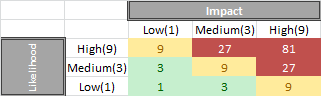
\includegraphics[scale=1.0]{Pictures/riskmatrix.png}
\caption{Risk Matrix}
\label{fig:riskmatrix}
\end{figure}

A risk matrix is shown in Table 1. The risks that lies in the upper right in red exceeds the level of tolerance and needs to be made action plan for. 
\subsection{Risk Log}
After the possible risks are identified, they are kept in table 2 following the priority of risk rating. The possible risks with high risk rating are marked in red and will be provided with an action plan below. 

\begin{table}[H]
\caption{Risk Log}
	\label{tab:risk}
	\begin{center}
		\begin{tabular}{|c|c|c|c|c|}
			\hline
			\makecell{\textbf{No.}} & \makecell{\textbf{Priority Hazard}} & \makecell{\textbf{Prob.}\\\textbf{(1-9)}} & \makecell{\textbf{Imp.}\\\textbf{(1-9)}} & \makecell{\textbf{Risk Rating}\\\textbf{(Prob.$\times$ Imp.)}} \\ \hline
			\makecell{1} & \makecell{ Estimates are inaccurat} & \makecell{9} & \makecell{9} & \makecell{\textcolor{red}{81}} \\
			\hline
			\makecell{2} & \makecell{ Code error } & \makecell{3} & \makecell{9} & \makecell{\textcolor{red}{27}} \\
			\hline
			\makecell{3} & \makecell{ Failure to follow the methodolog } & \makecell{3} & \makecell{9} & \makecell{\textcolor{red}{27}} \\
			\hline
			\makecell{4} & \makecell{ Preparation is inadequa } & \makecell{3} & \makecell{3} & \makecell{9} \\
			\hline
			\makecell{5} & \makecell{ Knowledge integratio} & \makecell{3} & \makecell{3} & \makecell{9} \\
			\hline
			\makecell{6} & \makecell{ Info loss during communicatio} & \makecell{3} & \makecell{3} & \makecell{9} \\
			\hline
			\makecell{7} & \makecell{ Ambiguous goa} & \makecell{1} & \makecell{9} & \makecell{9} \\
			\hline
			\makecell{8} & \makecell{ Disagreement with the coa} & \makecell{1} & \makecell{9} & \makecell{9} \\
			\hline
			\makecell{9} & \makecell{Low morale (interests lost)} & \makecell{1} & \makecell{9} & \makecell{9} \\
			\hline
			\makecell{10} & \makecell{ Tool selection proble} & \makecell{1} & \makecell{3} & \makecell{3} \\
			\hline
			\makecell{11} & \makecell{ Software collape} & \makecell{1} & \makecell{3} & \makecell{3} \\
			\hline
			\makecell{12} & \makecell{ Misunderstand the requiremen} & \makecell{1} & \makecell{3} & \makecell{3} \\
			\hline
		\end{tabular}
	\end{center}
	
\end{table}

\subsection{Action Plan}

An action plan is made for those risks with the highest likelihood and/or consequence. So the risks with risk rating above 9 are provided with the corresponding action plan.





%----------------------------------------------------------------------------------------
%	BIBLIOGRAPHY
%----------------------------------------------------------------------------------------

\bibliographystyle{ieeetr}
\bibliography{./Contents/References/references}

\newpage

\begin{appendices}
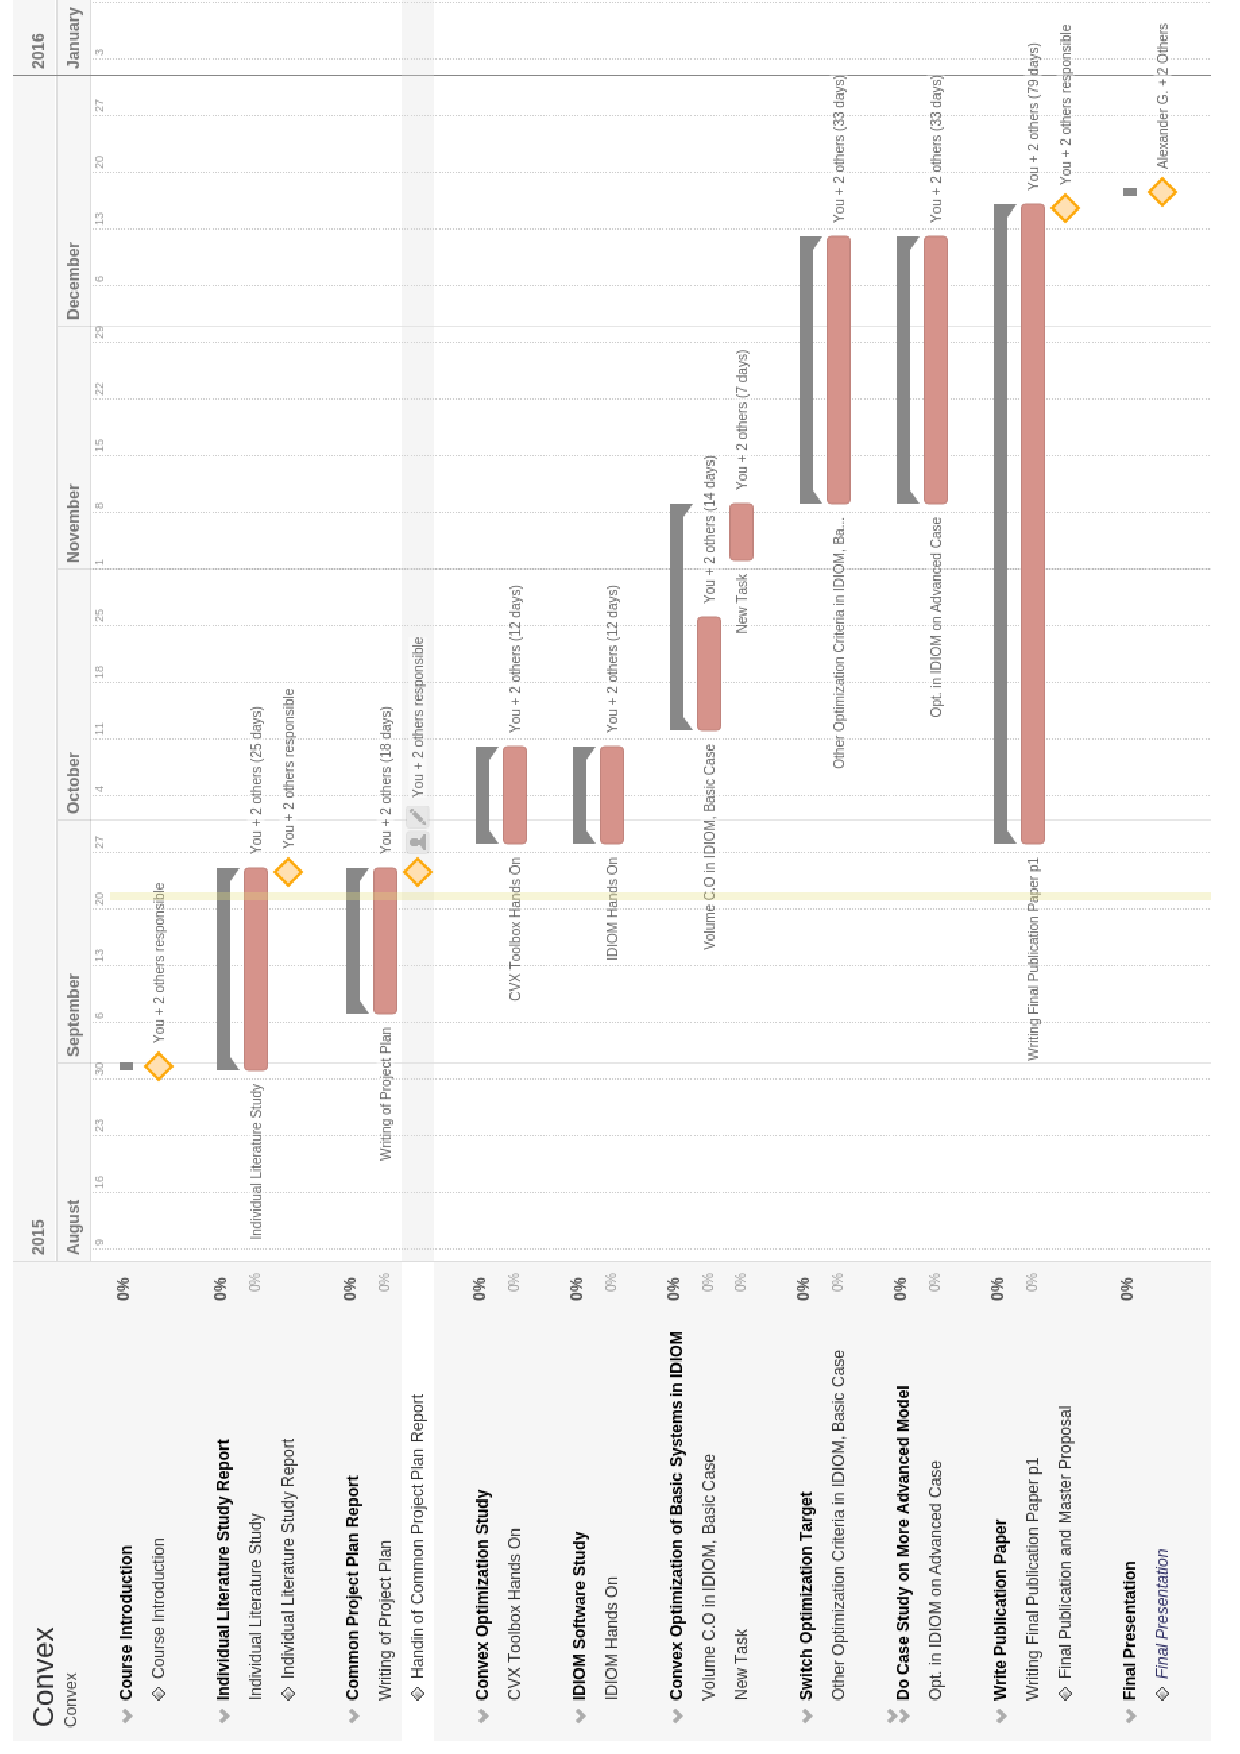
\includepdf[pages={1}]{./Contents/timeplan.pdf}
\end{appendices}
%----------------------------------------------------------------------------------------

\end{document}